% Options for packages loaded elsewhere
\PassOptionsToPackage{unicode}{hyperref}
\PassOptionsToPackage{hyphens}{url}
%
\documentclass[
]{article}
\usepackage{amsmath,amssymb}
\usepackage{lmodern}
\usepackage{ifxetex,ifluatex}
\ifnum 0\ifxetex 1\fi\ifluatex 1\fi=0 % if pdftex
  \usepackage[T1]{fontenc}
  \usepackage[utf8]{inputenc}
  \usepackage{textcomp} % provide euro and other symbols
\else % if luatex or xetex
  \usepackage{unicode-math}
  \defaultfontfeatures{Scale=MatchLowercase}
  \defaultfontfeatures[\rmfamily]{Ligatures=TeX,Scale=1}
\fi
% Use upquote if available, for straight quotes in verbatim environments
\IfFileExists{upquote.sty}{\usepackage{upquote}}{}
\IfFileExists{microtype.sty}{% use microtype if available
  \usepackage[]{microtype}
  \UseMicrotypeSet[protrusion]{basicmath} % disable protrusion for tt fonts
}{}
\makeatletter
\@ifundefined{KOMAClassName}{% if non-KOMA class
  \IfFileExists{parskip.sty}{%
    \usepackage{parskip}
  }{% else
    \setlength{\parindent}{0pt}
    \setlength{\parskip}{6pt plus 2pt minus 1pt}}
}{% if KOMA class
  \KOMAoptions{parskip=half}}
\makeatother
\usepackage{xcolor}
\IfFileExists{xurl.sty}{\usepackage{xurl}}{} % add URL line breaks if available
\IfFileExists{bookmark.sty}{\usepackage{bookmark}}{\usepackage{hyperref}}
\hypersetup{
  pdftitle={Getting Started With RMarkdown},
  pdfauthor={Cheng Peng},
  hidelinks,
  pdfcreator={LaTeX via pandoc}}
\urlstyle{same} % disable monospaced font for URLs
\usepackage[margin=1in]{geometry}
\usepackage{color}
\usepackage{fancyvrb}
\newcommand{\VerbBar}{|}
\newcommand{\VERB}{\Verb[commandchars=\\\{\}]}
\DefineVerbatimEnvironment{Highlighting}{Verbatim}{commandchars=\\\{\}}
% Add ',fontsize=\small' for more characters per line
\usepackage{framed}
\definecolor{shadecolor}{RGB}{248,248,248}
\newenvironment{Shaded}{\begin{snugshade}}{\end{snugshade}}
\newcommand{\AlertTok}[1]{\textcolor[rgb]{0.94,0.16,0.16}{#1}}
\newcommand{\AnnotationTok}[1]{\textcolor[rgb]{0.56,0.35,0.01}{\textbf{\textit{#1}}}}
\newcommand{\AttributeTok}[1]{\textcolor[rgb]{0.77,0.63,0.00}{#1}}
\newcommand{\BaseNTok}[1]{\textcolor[rgb]{0.00,0.00,0.81}{#1}}
\newcommand{\BuiltInTok}[1]{#1}
\newcommand{\CharTok}[1]{\textcolor[rgb]{0.31,0.60,0.02}{#1}}
\newcommand{\CommentTok}[1]{\textcolor[rgb]{0.56,0.35,0.01}{\textit{#1}}}
\newcommand{\CommentVarTok}[1]{\textcolor[rgb]{0.56,0.35,0.01}{\textbf{\textit{#1}}}}
\newcommand{\ConstantTok}[1]{\textcolor[rgb]{0.00,0.00,0.00}{#1}}
\newcommand{\ControlFlowTok}[1]{\textcolor[rgb]{0.13,0.29,0.53}{\textbf{#1}}}
\newcommand{\DataTypeTok}[1]{\textcolor[rgb]{0.13,0.29,0.53}{#1}}
\newcommand{\DecValTok}[1]{\textcolor[rgb]{0.00,0.00,0.81}{#1}}
\newcommand{\DocumentationTok}[1]{\textcolor[rgb]{0.56,0.35,0.01}{\textbf{\textit{#1}}}}
\newcommand{\ErrorTok}[1]{\textcolor[rgb]{0.64,0.00,0.00}{\textbf{#1}}}
\newcommand{\ExtensionTok}[1]{#1}
\newcommand{\FloatTok}[1]{\textcolor[rgb]{0.00,0.00,0.81}{#1}}
\newcommand{\FunctionTok}[1]{\textcolor[rgb]{0.00,0.00,0.00}{#1}}
\newcommand{\ImportTok}[1]{#1}
\newcommand{\InformationTok}[1]{\textcolor[rgb]{0.56,0.35,0.01}{\textbf{\textit{#1}}}}
\newcommand{\KeywordTok}[1]{\textcolor[rgb]{0.13,0.29,0.53}{\textbf{#1}}}
\newcommand{\NormalTok}[1]{#1}
\newcommand{\OperatorTok}[1]{\textcolor[rgb]{0.81,0.36,0.00}{\textbf{#1}}}
\newcommand{\OtherTok}[1]{\textcolor[rgb]{0.56,0.35,0.01}{#1}}
\newcommand{\PreprocessorTok}[1]{\textcolor[rgb]{0.56,0.35,0.01}{\textit{#1}}}
\newcommand{\RegionMarkerTok}[1]{#1}
\newcommand{\SpecialCharTok}[1]{\textcolor[rgb]{0.00,0.00,0.00}{#1}}
\newcommand{\SpecialStringTok}[1]{\textcolor[rgb]{0.31,0.60,0.02}{#1}}
\newcommand{\StringTok}[1]{\textcolor[rgb]{0.31,0.60,0.02}{#1}}
\newcommand{\VariableTok}[1]{\textcolor[rgb]{0.00,0.00,0.00}{#1}}
\newcommand{\VerbatimStringTok}[1]{\textcolor[rgb]{0.31,0.60,0.02}{#1}}
\newcommand{\WarningTok}[1]{\textcolor[rgb]{0.56,0.35,0.01}{\textbf{\textit{#1}}}}
\usepackage{longtable,booktabs,array}
\usepackage{calc} % for calculating minipage widths
% Correct order of tables after \paragraph or \subparagraph
\usepackage{etoolbox}
\makeatletter
\patchcmd\longtable{\par}{\if@noskipsec\mbox{}\fi\par}{}{}
\makeatother
% Allow footnotes in longtable head/foot
\IfFileExists{footnotehyper.sty}{\usepackage{footnotehyper}}{\usepackage{footnote}}
\makesavenoteenv{longtable}
\usepackage{graphicx}
\makeatletter
\def\maxwidth{\ifdim\Gin@nat@width>\linewidth\linewidth\else\Gin@nat@width\fi}
\def\maxheight{\ifdim\Gin@nat@height>\textheight\textheight\else\Gin@nat@height\fi}
\makeatother
% Scale images if necessary, so that they will not overflow the page
% margins by default, and it is still possible to overwrite the defaults
% using explicit options in \includegraphics[width, height, ...]{}
\setkeys{Gin}{width=\maxwidth,height=\maxheight,keepaspectratio}
% Set default figure placement to htbp
\makeatletter
\def\fps@figure{htbp}
\makeatother
\setlength{\emergencystretch}{3em} % prevent overfull lines
\providecommand{\tightlist}{%
  \setlength{\itemsep}{0pt}\setlength{\parskip}{0pt}}
\setcounter{secnumdepth}{-\maxdimen} % remove section numbering
\ifluatex
  \usepackage{selnolig}  % disable illegal ligatures
\fi

\title{Getting Started With RMarkdown}
\author{Cheng Peng}
\date{West Chester University}

\begin{document}
\maketitle

\hypertarget{section}{%
\section{}\label{section}}

\hypertarget{what-is-rmd}{%
\subsection{What is RMD}\label{what-is-rmd}}

R Markdown is a file format for making dynamic documents with R. An R
Markdown document is written in markdown (an easy-to-write plain text
format) and contains chunks of embedded R code, like the document below.

RMarkdown makes use of Markdown syntax. Markdown is a very simple
`markup' language that provides methods for creating documents with
headers, images, links, etc. from plain text files while keeping the
original plain text file easy to read.

R Markdown files are the source code for rich, reproducible documents.
We can transform an R Markdown file in two ways.

\begin{itemize}
\item
  \textbf{knit} - The rmarkdown package will call the \texttt{knitr}
  package. \texttt{knitr} will run each chunk of R code in the document
  and append the results of the code to the document next to the code
  chunk.
\item
  \textbf{convert} - The rmarkdown package will use the pandoc program
  to transform the file into a new format such as HTML, PDF, or
  Microsoft Word file. RMarkdown will preserve the text, code results,
  and formatting contained in the original.Rmd file.
\end{itemize}

The term \texttt{render} refers to the above two-step process of
knitting and converting an R Markdown file.

\hypertarget{create-an-rmarkdown-file}{%
\subsubsection{Create an RMarkdown
file}\label{create-an-rmarkdown-file}}

To create a new RMarkdown file (\texttt{.Rmd}), select
\texttt{File\ -\textgreater{}\ New\ File\ -\textgreater{}\ R\ Markdown}in
RStudio, then choose one of the file types we want to create.

The newly created.Rmd file comes with an RMarkdown template with basic
instructions.

\hypertarget{the-yaml-header}{%
\subsubsection{The YAML Header}\label{the-yaml-header}}

At the top of any RMarkdown script is a YAML (\texttt{Y}et
\texttt{A}nother \texttt{M}arkup \texttt{L}anguage) header section
enclosed by \texttt{-\/-\/-}. By default, this includes a title, author,
date and the file type you want to output to.

Many other options are available for different functions and formatting,
see here for .html options and here for .pdf options. Rules in the
header section will alter the whole document.

The following is the simplest YMAL template.

\begin{verbatim}
---
title: "Introduction to RMarkdown"
author: "Cheng Peng"
date: "12/25/2021"
output:
  html_document: default
  html_notebook: default
editor_options:
  chunk_output_type: inline
---
\end{verbatim}

Note that YAML is automatically generated that reflects the choice of
the file type and related file specifications. Therefore, we don't need
to know YAML unless we want to modify it manually.

\hypertarget{markdown-syntax}{%
\subsubsection{Markdown Syntax}\label{markdown-syntax}}

\begin{itemize}
\tightlist
\item
  \textbf{Formatting Text}

  \begin{itemize}
  \tightlist
  \item
    \emph{Italic} - single asterisk -\textgreater{} italic.
  \item
    \textbf{bold} - double asterisks -\textgreater{} bold face
  \item
    \texttt{code} - code in text
  \end{itemize}
\item
  \textbf{\texttt{Header}}

  \begin{itemize}
  \tightlist
  \item
    \texttt{\#\ Header\ 1}: single \texttt{\#} - level 1 header
  \item
    \texttt{\#\#\ Header\ 2}: double \texttt{\#\#}- level 2 header
  \item
    \texttt{\#\#\#\ Header\ 3}: triple \texttt{\#\#\#} - level 3 header
  \end{itemize}
\item
  \textbf{List}

  \begin{itemize}
  \tightlist
  \item
    \texttt{*\ Unordered\ list} - single asterisk \texttt{+}
    \textbf{space} -\textgreater{} unordered list
  \item
    \texttt{1.\ Ordered\ list} - numbered list
  \end{itemize}
\item
  \textbf{Hyperlink}

  \begin{itemize}
  \tightlist
  \item
    \texttt{\textless{}\ url\ \textgreater{}} - Example:
    \url{https://www.wcupa.edu/}
  \item
    \texttt{{[}link-name{]}(url)} - Example:
    \href{https://www.wcupa.edu/}{WCUPA}
  \end{itemize}
\item
  \textbf{LaTex Equations Syntax}

  \begin{itemize}
  \tightlist
  \item
    \texttt{\$\ LaTex\ commands\ \$} - Example:
    \(y = \beta_0 + \beta_1 x\)
  \end{itemize}
\end{itemize}

\hypertarget{code-chunks}{%
\subsection{Code Chunks}\label{code-chunks}}

Code that is included in .Rmd document should be enclosed by three
\texttt{backward\ apostrophes\ \textasciigrave{}\textasciigrave{}\textasciigrave{}\ (grave\ accents!)}.
These are known as code chunks. An executable code chunk looks like the
following.

\begin{Shaded}
\begin{Highlighting}[]
\CommentTok{\# code goes here}
\end{Highlighting}
\end{Shaded}

The first
line:\texttt{\textasciigrave{}\textasciigrave{}\textasciigrave{}\{r\ chunk-name-with-no-spaces\}}
contains the language (\texttt{r}) in this case, and the name of the
chunk, and other optional code chunk options. Next to the \{r\}, there
is a chunk name. The chunk name is not necessarily required however, it
is good practice to give each chunk a \texttt{unique} name to support
more advanced knitting approaches.

If the language is not specified in the curly bracket, the chunk is
simply a verbatim environment that keeps the content in the knitted
document. For example, the content in the following chunk will not be
executed.

\begin{verbatim}
The context will not be processed when converting this document to HTML, PDF, or other document formats.
\end{verbatim}

\hypertarget{code-chunk-options}{%
\subsubsection{Code Chunk Options}\label{code-chunk-options}}

There are a few options that can be used to control the graphical output
generated from the code in the code chunk. The following table lists a
few of them.

\hypertarget{inserting-graphics}{%
\subsection{Inserting Graphics}\label{inserting-graphics}}

There are two different ways to include images into RMD: Generated by
the code in the code chunk and external source of images.

\begin{itemize}
\tightlist
\item
  \textbf{R Generated Graphics}
\end{itemize}

Including R-generated graphics into RMD is straightforward. The
following example shows how to embed a graphic with some code chunk
options to layout the graphic.

\begin{Shaded}
\begin{Highlighting}[]
\FunctionTok{data}\NormalTok{(iris)}
\FunctionTok{pairs}\NormalTok{(iris[, }\SpecialCharTok{{-}}\DecValTok{5}\NormalTok{])}
\end{Highlighting}
\end{Shaded}

\begin{figure}

{\centering 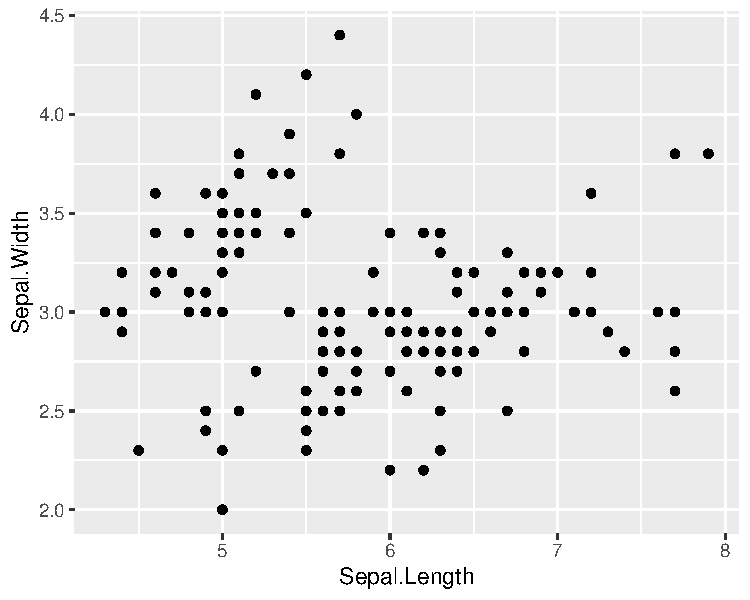
\includegraphics{w01-IntroRMD_files/figure-latex/unnamed-chunk-1-1} 

}

\caption{Pairwise scatter plot of iris data set}\label{fig:unnamed-chunk-1}
\end{figure}

\begin{itemize}
\tightlist
\item
  \textbf{External Images}
\end{itemize}

There are several ways to include an external image into RMD documents.

\begin{enumerate}
\def\labelenumi{\arabic{enumi}.}
\tightlist
\item
  Using HTML \texttt{img} Tag
\end{enumerate}

\begin{verbatim}
<br>
<center><img src="https://github.com/pengdsci/sta553/blob/main/image/boats.jpg?raw=true" alt="Portland Headlight" height="400" width="600"></center>
<br>
\end{verbatim}

\begin{enumerate}
\def\labelenumi{\arabic{enumi}.}
\setcounter{enumi}{1}
\tightlist
\item
  Using Markdown Syntax
\end{enumerate}

\texttt{!{[}caption{]}(path/to/image)}. In this case, we can set the
size of the image using the \texttt{width=} and/or \texttt{height=}.

\texttt{!{[}Portland\ Headlight{]}(https://github.com/pengdsci/sta553/blob/main/image/PortlandHeadlight.jpg?raw=true)\{width=70\%\}}

\begin{figure}
\centering
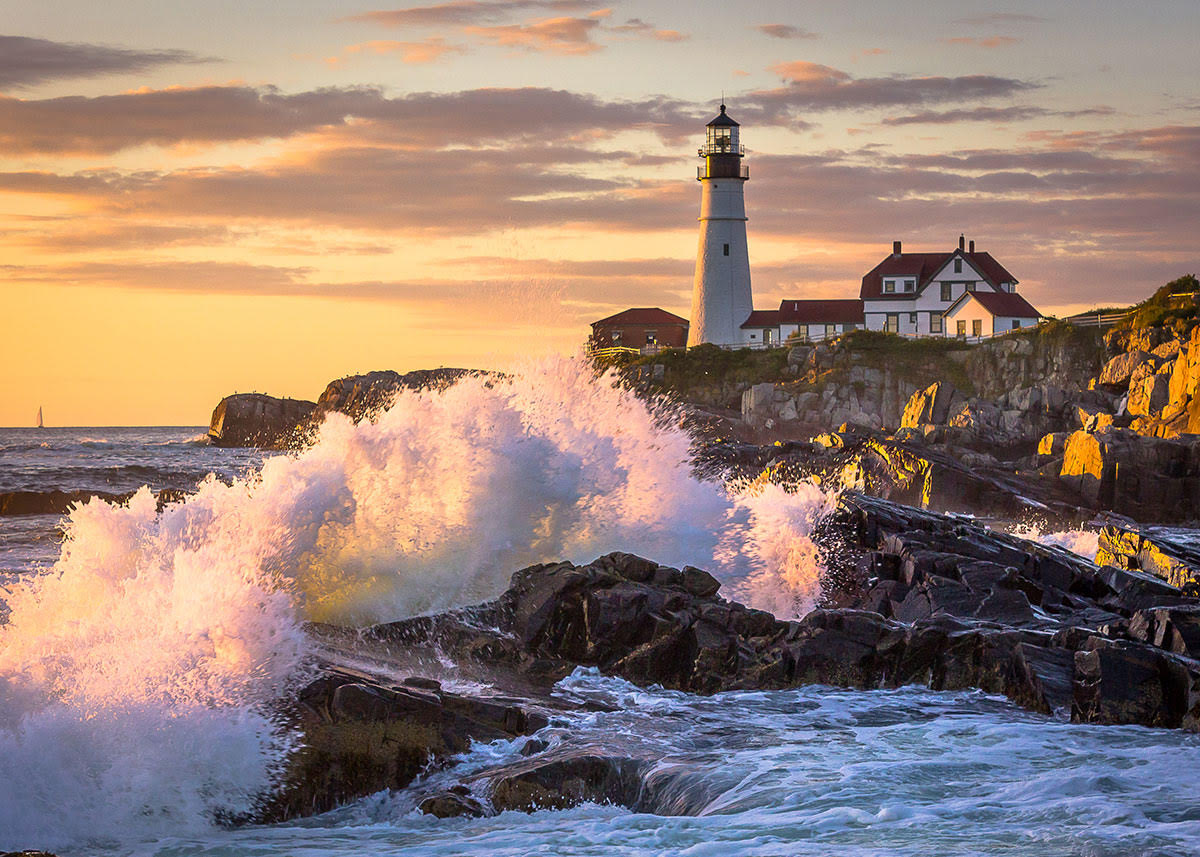
\includegraphics[width=0.7\textwidth,height=\textheight]{https://github.com/pengdsci/sta553/blob/main/image/PortlandHeadlight.jpg?raw=true}
\caption{Portland Headlight}
\end{figure}

Unfortunately, normal markdown image tags don't allow for any alignment
properties. Luckily, we can use HTML image tags to make enhance our
docs. For example, we can center the above image in our HTML document
using the following HTML tags.

\begin{verbatim}
<p align="center">
![Portland Headlight](https://github.com/pengdsci/sta553/blob/main/image/PortlandHeadlight.jpg?raw=true){width=70%}
</p>
\end{verbatim}

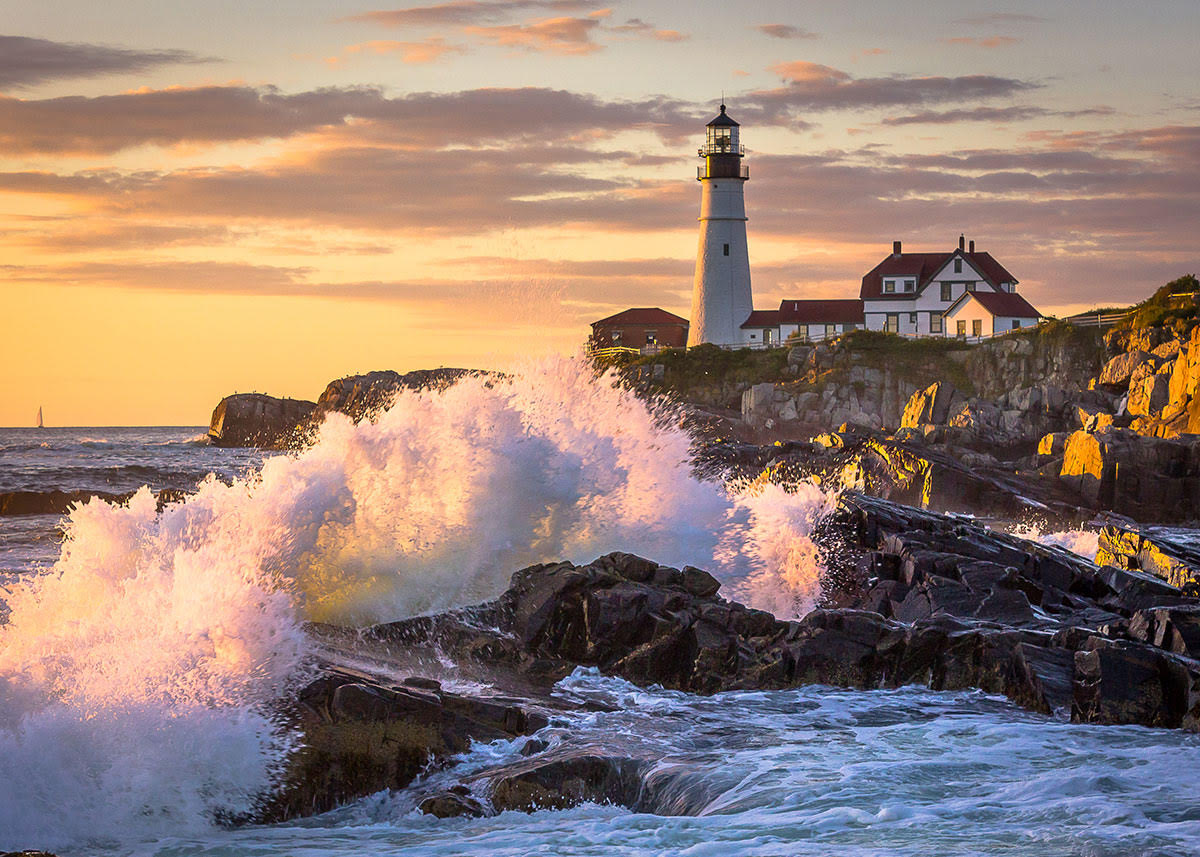
\includegraphics[width=0.7\textwidth,height=\textheight]{https://github.com/pengdsci/sta553/blob/main/image/PortlandHeadlight.jpg?raw=true}

\begin{enumerate}
\def\labelenumi{\arabic{enumi}.}
\setcounter{enumi}{2}
\tightlist
\item
  Using \texttt{knitr} Function
\end{enumerate}

\begin{verbatim}
## Chunk options: fig.align='center', echo=FALSE, fig.cap="White Mountain", out.width = '50%'
knitr::include_graphics("https://github.com/pengdsci/sta553/blob/main/image/WhiteMountain.jpg?raw=true")
\end{verbatim}

\begin{figure}

{\centering 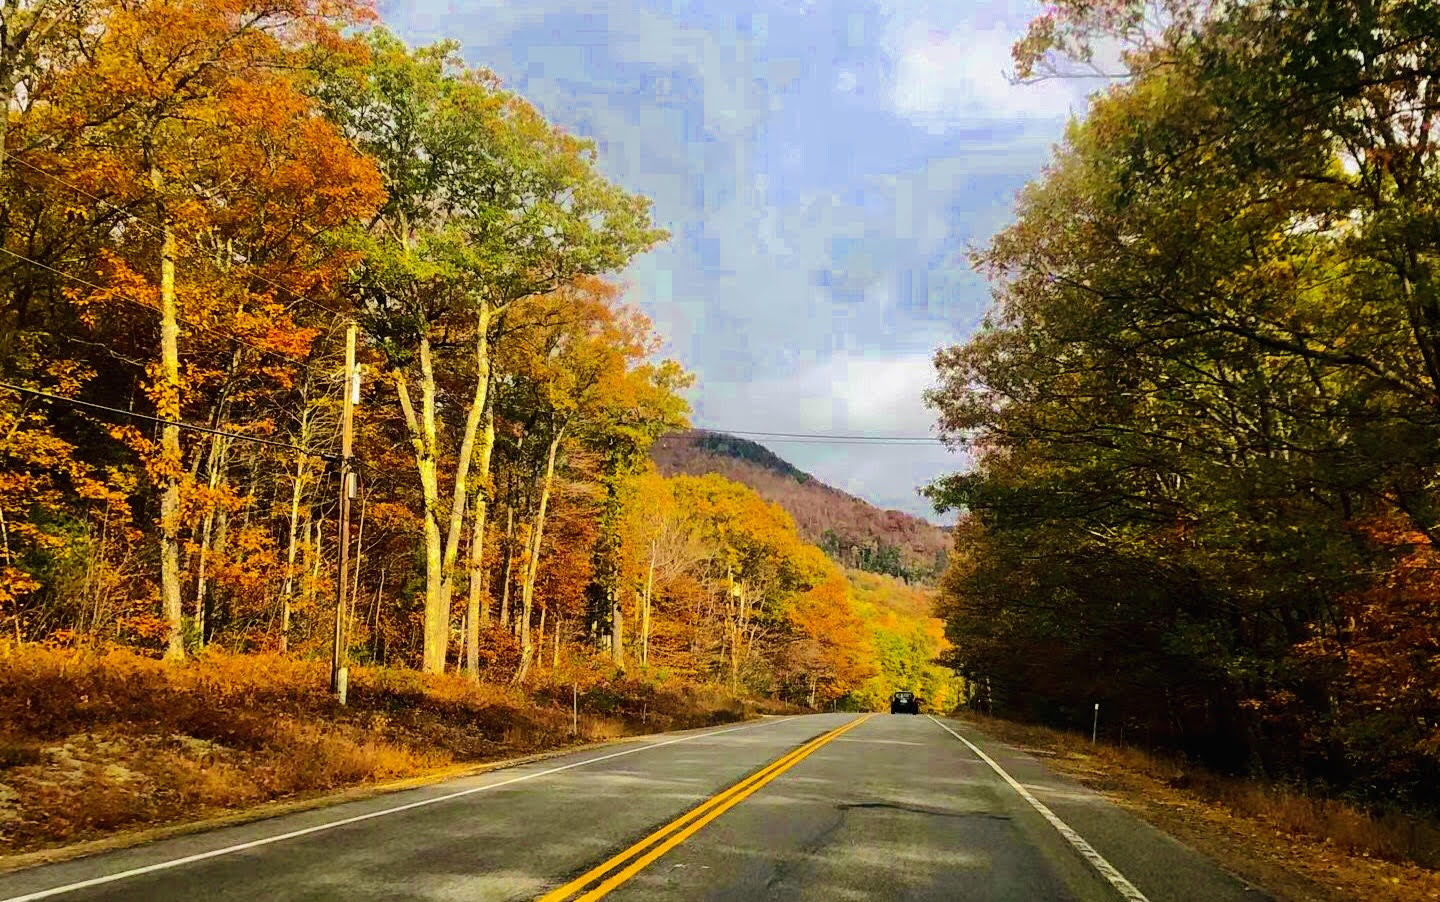
\includegraphics[width=0.5\linewidth]{https://github.com/pengdsci/sta553/blob/main/image/WhiteMountain.jpg?raw=true} 

}

\caption{White Mountain}\label{fig:unnamed-chunk-2}
\end{figure}

\hypertarget{inserting-tables}{%
\subsection{Inserting Tables}\label{inserting-tables}}

A quality table is also an important visualization tool. We introduce
three methods for inserting nice-looking tables into the RMD document.

\begin{itemize}
\tightlist
\item
  \textbf{Extracting R Output Matrix Using \texttt{kable()} Function}
\end{itemize}

For example, we fit a linear regression model using iris data and
extract the statistics of model fit to define a table.

\begin{Shaded}
\begin{Highlighting}[]
\FunctionTok{data}\NormalTok{(iris)}
\NormalTok{iris.model }\OtherTok{=} \FunctionTok{lm}\NormalTok{(Sepal.Length}\SpecialCharTok{\textasciitilde{}}\NormalTok{., }\AttributeTok{data =}\NormalTok{ iris)  }\CommentTok{\# fit a linear model}
\NormalTok{mod.stats }\OtherTok{=} \FunctionTok{coef}\NormalTok{(}\FunctionTok{summary}\NormalTok{(iris.model))         }\CommentTok{\# inferential stats of coefficients}
\FunctionTok{kable}\NormalTok{(mod.stats)   }\CommentTok{\# }
\end{Highlighting}
\end{Shaded}

\begin{longtable}[]{@{}lrrrr@{}}
\toprule
& Estimate & Std. Error & t value &
Pr(\textgreater\textbar t\textbar) \\
\midrule
\endhead
(Intercept) & 2.1712663 & 0.2797942 & 7.760228 & 0.0000000 \\
Sepal.Width & 0.4958889 & 0.0860699 & 5.761466 & 0.0000000 \\
Petal.Length & 0.8292439 & 0.0685276 & 12.100867 & 0.0000000 \\
Petal.Width & -0.3151552 & 0.1511958 & -2.084418 & 0.0388883 \\
Speciesversicolor & -0.7235620 & 0.2401689 & -3.012721 & 0.0030596 \\
Speciesvirginica & -1.0234978 & 0.3337263 & -3.066878 & 0.0025843 \\
\bottomrule
\end{longtable}

\begin{itemize}
\tightlist
\item
  \textbf{Markdown Table}
\end{itemize}

We can manually create a Markdown table. See the following example.

\begin{verbatim}
| Plant | Temp. | Growth |
|:------|:-----:|-------:|
| A     | 20    | 0.65   |
| B     | 20    | 0.95   |
| C     | 20    | 0.15   |
\end{verbatim}

The resulting Markdown has the following

\begin{longtable}[]{@{}lcr@{}}
\toprule
Plant & Temp. & Growth \\
\midrule
\endhead
A & 20 & 0.65 \\
B & 20 & 0.95 \\
C & 20 & 0.15 \\
\bottomrule
\end{longtable}

The Markdown table syntax is explained in the following:

\begin{itemize}
\tightlist
\item
  \texttt{:-\/-\/-\/-:}: Centre
\item
  \texttt{:-\/-\/-\/-\/-}: Left
\item
  \texttt{-\/-\/-\/-\/-:}: Right
\item
  \texttt{-\/-\/-\/-\/-\/-}: Auto
\end{itemize}

\hfill\break

\hfill\break

\begin{itemize}
\tightlist
\item
  \textbf{HTML Table}
\end{itemize}

\begin{verbatim}
<table border = 1>
  <tr>
    <th>Company</th>
    <th>Contact</th>
    <th>Country</th>
  </tr>
  <tr>
    <td>Alfreds Futterkiste</td>
    <td>Maria Anders</td>
    <td>Germany</td>
  </tr>
  <tr>
    <td>Centro comercial Moctezuma</td>
    <td>Francisco Chang</td>
    <td>Mexico</td>
  </tr>
</table>
\end{verbatim}

A basic HTML table

Company

Contact

Country

Alfreds Futterkiste

Maria Anders

Germany

Centro comercial Moctezuma

Francisco Chang

Mexico

\begin{itemize}
\tightlist
\item
  \textbf{LaTex Table}
\end{itemize}

This will not work if we knit the RMD to HTML since it is a LaTex table.

\begin{verbatim}
\begin{table}
\centering
\begin{tabular}{llll}
1 & 2 & 3 & 4  \\
1 & 3 & 4 & 6  \\
3 & 4 & 1 & 8  \\
5 & 2 & 0 & 1 
\end{tabular}
\end{table}
\end{verbatim}

\hypertarget{creating-pdf}{%
\subsection{Creating PDF}\label{creating-pdf}}

Creating \texttt{.pdf} documents for printing in A4 requires a bit more
fiddling around. RStudio uses another document compiling system called
LaTeX to make \texttt{.pdf} documents.

The easiest way to use LaTeX is to install the \texttt{TinyTex}
distribution from within RStudio. First, restart the R session (Session
-\textgreater{} Restart R), then run these lines in the console:

\begin{verbatim}
install.packages("tinytex")
tinytex::install_tinytex()
\end{verbatim}

Becoming familiar with LaTeX will give you a lot more options to make
your R Markdown .pdf look pretty, as LaTeX commands are mostly
compatible with R Markdown, though some googling is often required.

To install a full-functioning LaTex, MikTex is recommended. The official
website for MikTex is \url{https://miktex.org/download}.

We can also choose different options to make a nicer PDF by clicking the
arrow on the gear sign () and then selection
\texttt{Output\ Options...}. Then select \textbf{Output Format:} as
\texttt{PDF}. Then we can choose appropriate options.

\hypertarget{miscellaneous}{%
\subsection{Miscellaneous}\label{miscellaneous}}

We have introduced the basics of R Markdown. Several good features are
worth mentioning.

\hypertarget{markdown-presentations}{%
\subsubsection{Markdown Presentations}\label{markdown-presentations}}

R Markdown can prepare presentations in HTML slides, PDF Beamer, and
Microsoft PowerPoint Presentation. Some of the lecture notes will be
prepared in PDF Beamer.

\hypertarget{shiny-apps-and-rmarkdown}{%
\subsubsection{Shiny Apps and
RMarkdown}\label{shiny-apps-and-rmarkdown}}

A recent development is the ability to put Shiny elements into an
RMarkdown document.

These documents, again, need a Shiny server to run, but take advantage
of the easy formatting of RMarkdown to present the user interface -
server and UI elements sit in the same document.

\begin{itemize}
\tightlist
\item
  \textbf{RMarkdown} - supplies the HTML instead of a \texttt{ui.R}
  file.
\item
  \textbf{Shiny} - supplied reactive components within your RMarkdown
\end{itemize}

We will prepare shiny lecture notes using RMarkdown in this class.

\hypertarget{working-directory}{%
\subsubsection{Working Directory}\label{working-directory}}

Sometimes we may want to use a specific directory as the working
directory to store relevant files associated with the same analysis. The
usual way to change the working directory is \texttt{setwd()},
\textbf{but} please note that \texttt{setwd()} is not persistent in R
Markdown (or other types of knitr source documents), which means
\texttt{setwd()} only works for the current code chunk, and the working
directory will be restored after this code chunk has been evaluated.

It is not encouraged to use \texttt{setwd()} in RMarkdown documents.

\hypertarget{css-style}{%
\subsubsection{CSS Style}\label{css-style}}

We can include a CSS-style file to format HTML. The style file used in
this RMD is given below.

\begin{verbatim}
<style type="text/css">
div#TOC li {
    list-style:none;
    background-image:none;
    background-repeat:none;
    background-position:0;
}
h1.title {
  font-size: 24px;
  color: darkRed;
  text-align: center;
}
h4.author { /* Header 4 - and the author and data headers use this too  */
    font-size: 18px;
  font-family: "Times New Roman", Times, serif;
  color: DarkRed;
  text-align: center;
}
h4.date { /* Header 4 - and the author and data headers use this too  */
  font-size: 18px;
  font-family: "Times New Roman", Times, serif;
  color: DarkBlue;
  text-align: center;
}
h1 { /* Header 3 - and the author and data headers use this too  */
    font-size: 22px;
    font-family: "Times New Roman", Times, serif;
    color: darkred;
    text-align: center;
}
h2 { /* Header 3 - and the author and data headers use this too  */
    font-size: 18px;
    font-family: "Times New Roman", Times, serif;
    color: navy;
    text-align: left;
}
h3 { /* Header 3 - and the author and data headers use this too  */
    font-size: 15px;
    font-family: "Times New Roman", Times, serif;
    color: darkred;
    font-face: bold;
    text-align: left;
}
h4 { /* Header 4 - and the author and data headers use this too  */
    font-size: 18px;
    font-family: "Times New Roman", Times, serif;
    color: darkred;
    text-align: left;
}
</style>
\end{verbatim}

\end{document}
